\chapter{Introduction}
\label{chap:Intro}
The sun is the primary source of energy for Earth, and is essential for photosynthesis in plants, which forms the basis of most food chains, and for driving the weather and climate systems that shape our environment. Its consistent radiation supports all life forms, regulates global temperatures, and influences fundamental ecological and biological processes that are vital for the Earth's diverse ecosystems. From the very outset of human life, the sun has been a subject of profound admiration, occupying a central role in various religious beliefs and was often synonym of an incomparably vast and potent source of energy. It was not until the beginning of the twentieth century that progress in particle physics allowed to unravel the secret of solar energy: nuclear fusion. It is the physical process where two light atoms merge to form a heavier atom, releasing significant energy as a result of mass-to-energy conversion. The strong nuclear force is fundamental to confine the positively charged protons with neutrons in an atomic nucleus. Every element is characterized by its total binding energy, that corresponds to the energy needed to break an atom into its constituting protons and neutrons. A higher total binding energy means that the element is more stable. The maximum binding energy is observed for iron ($^{56}Fe$), it means that (roughly) all lighter elements can produce energy by fusion and heavier by fission, as it is done in conventional nuclear power plants.  \newline 

The dream of achieving nuclear fusion in a laboratory to produce energy emerged shortly thereafter. In today's climate crisis, nuclear fusion is even more appealing because it does not emit carbon emissions, does not present the risk of a catastrophic meltdown and its fuel, hydrogen, is readily available. Since replicating the sun's core conditions on Earth, particularly the immense pressure, is not feasible, alternative approaches were searched. A look at Fig. \ref{fig:Intro_fusionCrossSections} with the reaction cross-section of various pairs of light atoms shows that deuterium-tritium (D-T) fusion has the highest likelihood at the most accessible temperature. These two hydrogen isotopes are hence the most favorable candidates for fusion and rhe reaction reads: \newline

\begin{equation}
	^2_1D + ^3_1T \rightarrow ^4_2He [3.5MeV] + ^1_0n [14.1 MeV]
\end{equation}

In the fusion reaction between deuterium and tritium, one alpha-particle (or Helium-4 nucleus) and one neutron are produced. 80\% of the released energy is carried by the neutron. Deuterium is a naturally abundant isotope of hydrogen, but tritium, which is radioactive and has a relatively short half-life time of 12 years, must be produced artificially. The most widely used method to obtain tritium is via neutron activation of lithium-6, but this requires either a nuclear power plant or another type of effective neutron source. As each fusion reaction emits one neutron, all future D-T reactor designs rely on a yet-to-be-tested technology to produce tritium inside the reactor, in the so-called "tritium breeding" process. To compensate inevitable particle losses, the neutron flux is first multiplied by hitting a layer of beryllium or lead. The neutrons then react with the lithium in an exothermic reaction, releasing one new tritium and one helium atom. The limiting resource for a large-scale deployment of nuclear fusion for power generation is then lithium, but even then, the required quantities are well below the current extraction for industrial needs. \\


\begin{figure}[H]
	\centering
	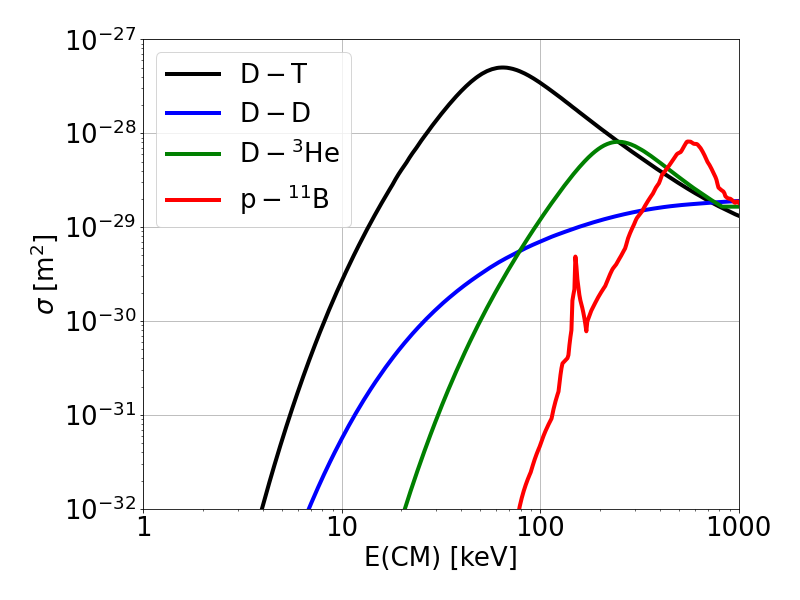
\includegraphics[width=0.62\textwidth]{schemes/fusion-xsecs2.png}
	\caption{Fusion reaction cross-sections for the most promising pairs of light elements over center-of-mass energy.}
	\label{fig:Intro_fusionCrossSections}
\end{figure}


At the very high temperatures needed for nuclear fusion, the electromagnetic force is insufficient to maintain the cohesion of electrons and their atomic nuclei, resulting in the formation of a state of matter known as plasma. Plasma is an ionized gas composed of positively charged nuclei and negatively charged electrons, which interact electromagnetically. \newline

Lawson's criterion \cite{Lawson1957} estimates the necessary plasma conditions to reach the break-even point, where fusion power exceeds heating and conduction losses. For D-T fusion, the triple product of density $n$, temperature $T$, and energy confinement time $\tau_E$ must exceed:

\begin{equation}
	\label{eq:LawsonCriterionDT}
	nT\tau_E > 10^{-21} \, \text{keV} \cdot \text{m}^{-3} \cdot \text{s}
\end{equation}

From a practical point of view, an important metric is the fusion gain $Q$, which measures the ratio of power produced in the nuclear fusion reaction to the required heating power to maintain plasma conditions. One major milestone is the break-even point, when the fusion reaction produces enough power to maintain a steady state at $Q=1$. However, the plasma can only capture a fraction of the produced fusion energy, as most fast neutrons rapidly escape the plasma, with, as seen before, 80\% of the energy. Therefore, external heating is still required until $Q>5$. Past this point, fusion produces more heat than the total required heating power and sustains itself in a state known as ignition ($Q=\infty$). Commercial operation of fusion power plants requires reliable access to ignition, which still requires decades of research. \\

The reaction cross-section determines an optimal temperature of approximately 15-40 keV (~150 million °C) for D-T fusion reactions, leading fusion reactor designs to maximize either of the two remaining parameters: density or confinement time. There is a large variety of approaches to artificial fusion, but today, two concepts show the most promise. Inertial Confinement Fusion (ICF) seeks to compress dense fuel pellets for an extremely brief duration using high-powered lasers. Conversely, Magnetic Confinement Fusion (MCF) utilizes strong magnetic fields to sustain stable plasmas at relatively low densities. Within MCF, there are two primary designs: tokamaks, which use a toroidal chamber with an axisymmetric magnetic field, and stellarators, which use a twisted magnetic configuration to improve plasma confinement.\\

\begin{figure}[H]
	\centering
	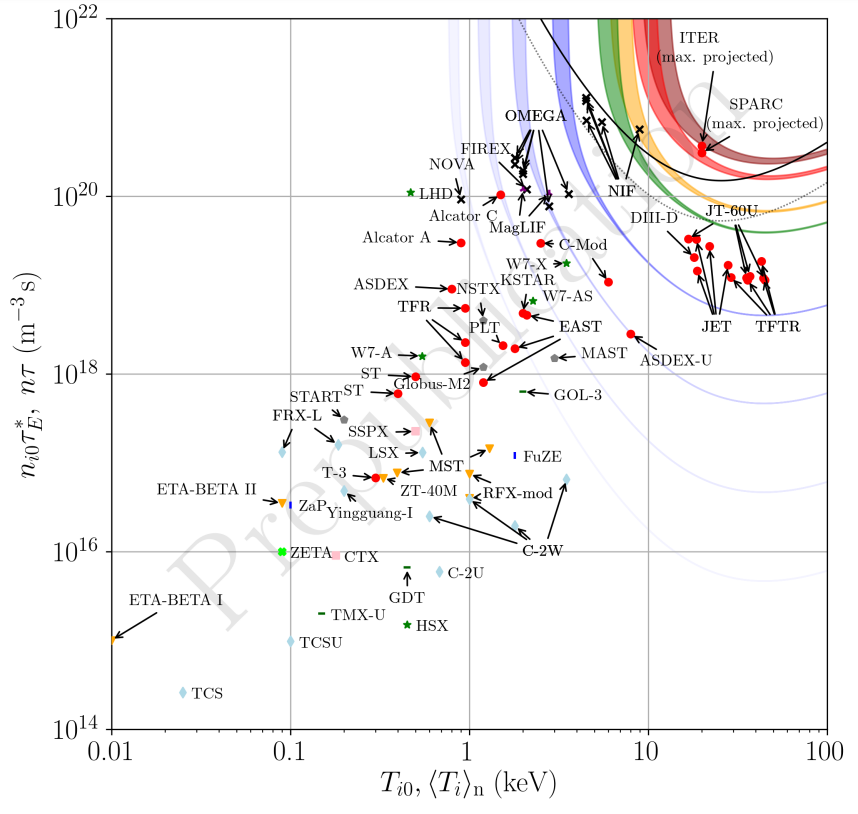
\includegraphics[width=0.7\textwidth]{schemes/Fusion_Triples_2021.png}
	\caption{Relation of the fusion trapping $n\tau_E$ to the temperature in current and future devices. For MCF The break-even point (Q=1) corresponds to the green area and ignition (Q=$\infty$) is brown. Ignition for ICF is reached at the solid black line. Taken from \cite{wurzel2022progress}}
	\label{fig:Intro_fusionTripleProduct}
\end{figure}

Figure \ref{fig:Intro_fusionTripleProduct} depicts the current status of fusion experiments with respect to Lawson's criterion. On December 5, 2022, the National Ignition Facility (NIF) reached the break-even point for the first time, achieving a 3.1 MJ fusion yield with 2 MJ of injected laser power\cite{abu2024achievement}. Large MCF devices, such as DIII-D, TFTR, JET, and JT60-SA, are already very close to the break-even point. Next-generation devices, including ITER and SPARC, which are under construction, are expected to achieve $Q>1$. \\


In this work, we focus on the most promising candidate for MCF, the tokamak. The three Soviet physicists Lavrent'ev, Sakharov, and Tamm had the idea in the early 1950s \cite{azizov2012tokamaks} to confine the plasma in a strong toroidal magnetic field. Additional coils create a poloidal field to suppress instabilities, such that plasma particles are trapped on helical trajectories. The first experiment was conducted in 1954 at the LIPAN institute in Moscow, the predecessor of the Kurchatov institute. The term "tokamak" or "\cyrillic{токамак}" was coined in 1957 by Golovin, and is a Russian acronym of "\cyrillic{тороидальная камера с магнитными катушками}", which translates to "toroidal chamber with magnetic coils," where the "G" from "mag" was transformed to "K" for better sonority \cite{shafranov1999trends}. \\

Since then, tokamaks gained popularity in the USSR and abroad. The design was improved with each generation of new devices to operate at ever higher power. In the 1960s, the first devices surpassed the Bohm limit. Technological progress in plasma heating and superconducting coils led to second-generation tokamaks, such as TFTR and JET, which could operate at much higher temperatures and magnetic field strengths. Another breakthrough was the refined shaping of the magnetic equilibrium with the introduction of divertors to carefully direct particle fluxes, which ultimately culminated in the discovery of the high-confinement (H) mode, allowing for much higher core temperatures. The largest fusion experiment, ITER, is currently under construction in southern France by an international collaboration of seven member parties. At full operation, it is expected to achieve ignition, a state where the fusion reaction emits sufficient radiation to maintain plasma conditions. Its scientific goals include maintaining burning plasma for an extended period of time and demonstrating safe operation in the nuclear phase. It will also serve as a test facility for tritium breeding blankets, a much-needed technology to produce tritium in situ. Currently, tritium is only obtained in pressurized water reactors, and the worldwide annual production of about 500 g is far insufficient to meet the required 55.8 kg per GW installed in a fusion power plant\cite{abdou2020physics}. \\

Understanding fundamental physical processes in the plasma still constitutes an important part of today's research on fusion energy. With the harsh conditions inside the tokamak vessel, diagnostics can only measure indirect plasma properties and are limited in spatial resolution. Simulations are then essential to interpret and extend the findings from experimental data and understand the correlations between different observations. They support current tokamak operation with estimates of heat deposition, wall erosion, and by predicting plasma disruptions. For the design of future fusion devices, simulations allow the evaluation of new magnetic configurations and the optimization of these designs. One particular region of interest is the transition from the hot core region, with closed magnetic field lines, to the edge and the scrape-off layer, where particles traveling along the magnetic field collide with the physical wall in the divertor region. Strong temperature gradients lead to large turbulent structures, driven by resistive drift waves. It is crucial to understand the dynamics and interactions with impurities or neutrals, as fluxes crossing the separatrix largely define the quality of plasma confinement. From a material design perspective, edge plasma simulations are essential to characterize the particle and heat fluxes on the physical wall. \\

The mechanisms at play at the plasma boundary result from the complex interplay of transport processes in the plasma, losses at the wall, and complex atomic and molecular interactions. In this region, particles experience very fast transport along the magnetic field lines and slower, often turbulence-driven, anomalous cross-field transport\cite{loarte2007}. The ratio between these phenomena characterizes the decay length of density and temperature profiles, which further determine the confinement quality of the core plasma and the total heat exhaust on the divertor target. Drift-reduced fluid models are particularly suited to simulate tokamak edge plasma, as they focus on low-frequency dynamics dominating the turbulent transport. The simplifications make it numerically feasible to simulate plasma behaviour over relevant time scales with still accurate results. Major simulation frameworks that follow this approach include GRILLIX\cite{GrillixGeneralPaper,stegmeir2019}, GBS\cite{Ricci_2012,giacomin2022gbs}, BOUT++\cite{DUDSON_2009,dudson2015} or SOLEDGE3X\cite{tamain2016tokam3x,Bufferand_2021}. \\

In the scope of this thesis, I extended the physical model underlying the SOLEDGE3X code, originally developed at CEA Cadarache. In its current version, turbulent simulations are limited to L-modes and small machines due to numerical issues and a limited model for larger machines. A significant limitation arises from the anisotropy between the parallel (resistive) and perpendicular (from the time evolution of the vorticity) Laplacians acting on the electric potential. This becomes problematic when the resistivity is very small. Even in the electrostatic collisional regime found in the plasma edge, electron inertia and electromagnetic effects play a substantial role, especially as electron inertia replaces resistivity as it approaches zero. \\

As the plasma approaches the L-H transition, electromagnetic effects become increasingly important. The H-mode is characterized by a suppression of cross-field transport due to "ExB" drifts, which are partially replaced by electromagnetic transport. Significant magnetic reconnection processes lead to important transport of plasma particles from the hot core to the cold edge, with radial fluxes still below "ExB" advection, but non-negligible in understanding the overall plasma behavior. \\

This thesis is dedicated to the implementation of an electromagnetic model within SOLEDGE3X, which includes magnetic induction in the parallel electric field, perturbations of the magnetic equilibrium (flutter), and a finite electron mass in Ohm's law. This development pursues several goals: first, it improves the accuracy of the physical model; second, it enhances numerical robustness by mitigating the poor matrix conditioning associated with low resistivity; and third, it extends the capabilities of SOLEDGE3X to study turbulence and transport in larger machines and for higher-power scenarios. \\

!!!!!!! PRESENT CHAPTERS OF THE THESIS !!!!!!!!!!

